\documentclass[a4paper, 12pt]{article}

\usepackage[french]{babel} 
\usepackage[utf8]{inputenc}
\usepackage[T1]{fontenc} 
\usepackage{amsmath}
\usepackage{amssymb}
\usepackage{listings}  
\usepackage{graphicx}
\usepackage[margin=2.5cm]{geometry}

\author{David \bsc{Haven} \and Eddy \bsc{Ndizera} \and Ivan \bsc{Ahad} \and Julien \bsc{Sterbelle}}

\title{Rapport Projet MCP}

\date{\today}

\begin{document}

\maketitle
\section{Introduction}

Dans le cadre du cours Méthode de Conception de Programmes, il nous a été demandé de construire un algorithme \textit{correct} qui prend en entrée un \textbf{cadran $C_{1}$} et un \textbf{entier naturel $n$} et qui génère le cadran résultant de la rotation de longueur $n$ de $C_{1}$ . \newline

L'algorithme doit répondre à certaines contraintes qui sont:
\begin{itemize}
\item il doit être le plus général possible;
\item il doit être le plus simple possible;
\item il ne doit pas utiliser d'Api Java;
\item la mémoire utilisée doit être fixe;
\item il doit avoir une complexité algorithmique temporelle en $O(n)$ où $n$ représente la taille du cadran. \newline
\end{itemize}

Ce présent rapport a donc pour but de vous présenter notre solution au problème et de vous prouvez que notre algorithme est \textbf{correct} et qu'il répond aux \textbf{contraintes} citées plus haut. Pour ce faire, la méthode utilisée est celle vue en cours qu'on peut découper en plusieurs parties:
%Expliquer différentes parties ?
\begin{itemize}
\item Théorie du problème
\item Convention de représentation
\item Spécifications des méthodes
\item Code Java
\item Correction totale de l'algorithme: triplet de Hoare-Manna et variant \newline
\end{itemize}

\section{Théorie du problème}

Soit $C$ un cadran de longueur $y$ (disposant de y éléments). Nous voulons effectuer une rotation de  longueur $n$ sur ce cadran. Une première propriété utile à la résolution de ce problème est la théorie des \textbf{modulos}. \newline

La théorie des modulos nous permet de dire, si on compte les éléments du cadran à partir de l'indice 0, de dire que l'élément 0 est le même que le yème élément pour le cadran C. L'élément 1 est égal au (y+1)éme élément du cadran C, etc. On peut le traduire sous cette écriture:\newline
i mod y = y+i mod y ou de façon plus générale \newline
i mod y = (k*y)+i mod y (où i est compris entre [0, y[ et k appartient aux entiers naturels). \newline
%Introduire schéma pour montrer cela

La deuxième théorie est la suivante:\newline
Soit $p$ le \textbf{plus grand commun diviseur} de $y$ et $n$. Nommons $a_{0}$, $a_{1}$, ..., $a_{y-1}$ les éléments du cadran. Considérons un \textbf{parcours} du cadran par pas de $n$ en démarrant de l'élément $a_{i}$ ($i \in [0,y[$) comme étant la suite d'éléments $a_{i}$ , $a_{i+n}$,$a_{i+2n}$, ... du cadran jusqu'à retomber sur l'élément de départ $a_{i}$. \newline

Nous pouvons donc énoncer la théorie du problème comme étant que les \textbf{parcours successifs} par pas de $n$ avec point de départ les éléments  $a_{i}$, ..., $a_{i+(p-1)}$ permet de visiter tout les éléments du cadran une fois sauf les éléments de départ qui seront visités au début et à la fin d'un parcours.\newline

La démonstration de cette propriété se fera en 2 parties:
\begin{itemize}
\item Montrer que chaque parcours contiendra un même \textbf{nombre d'éléments} $k+1$, où $k = y/p$.
\item Montrer que les parcours avec point de départ $a_{i}$,...,$a_{i+(p-1)}$ ne possèdent \textbf{aucun élément en commun}.\newline
\end{itemize}

Soit $k = y/p$. Pour un parcours $P$ quelconque ayant comme point de départ $a_{i}$ et pour pas $n$, il faut avoir effectuer $k$ nombre de pas de n avant de retomber sur $a_{i}$. \newline

En effet, si nous visitons les éléments par pas de $n$, il faut que la somme des pas soit égale à un multiple de $y$ pour retomber sur un même élément (on peut démontrer cela gràce aux modulos, pour que 2 nombres modulo n soit égaux il faut que leur différence soit un multiple de n). Or $n*k$ est bien un multiple de y puisque $k = y/p$ et que $p$ divise $n$. On peut résumer cela par la formule:\newline
$(n*k+i)$ mod $y = i$ \newline

Il reste à prouver que $n*k$ est bien le plus petit multiple de $y$ divisible par $n$. On a que:\newline
$nk = \frac{n*y}{p} = q*y$ (où $n=q*p$).\newline
Il n'existe pas de multiple de $y$ divisible par $n$ plus petit que $n*k$ car sinon $p$ ne serait pas le plus grand commun diviseur de $y$ et $n$.\newline

On peut conclure que chaque parcours contient alors $k+1$ éléments. \newline

Nous allons maintenant prouver que chaque éléments sont différents pour les parcours commençant à l'indice $a_{i}$ jusqu'aux parcours commençant à l'indice $a_{i+(p-1)}$.\newline

Considérons deux parcours $P_{1}$ et $P_{2}$ ayant respectivement comme point de départ $a_{i}$ et $a_{j}$ avec $0 \leq i < j \leq p-1$. Pour que les parcours $P_{1}$ et $P_{2}$ contiennent un élément en commun, il faudrait qu'il existe un élément dans le cadran tel que:\newline
$(n*t_{1})+i$ mod $y = (n*t_{2})+j$ mod $y$  (où $t_{1}$ et $t_{2}$ sont des entiers naturels)\newline
$\Leftrightarrow (n(t_{1} - t_{2})$ mod $y = j-i$ mod $y$ \newline

Si on divise les 2 membres par $p$, on obtient alors:\newline
$q(t_{1} - t_{2}) = \frac{j-i}{p}$  (où $n=q*p$).\newline

On a que $(j-i) < p$. De plus comme $i < j$, on peut supposer que $t_{1} > t_{2}$. Comme $(t_{1}-t_{2}) \geq 1$ et que $(\frac{j-i}{p}) < 1$ alors on peut conclure que cette égalité n'a aucune solution et que donc il n'y a pas d'éléments en commun pour les parcours cités plus haut.\newline

On vient de démontrer que la propriété énoncée est vraie. Comme chaque parcours contient $k = y/p$ éléments différents et qu'on effectue $p$ parcours de cette sorte en changeant d'indice de départ, on a bien qu'on visite $k*p = (y*p)/p = y $ éléments différents. Donc on aura visité tout les éléments du cadran. \newline

A cela s'ajoute une autre propriété qui découle de la dernière qui est qu'on peut décaler tout les éléments du cadran après y sauts (où un saut est un pas de n). En effet, cela revient, pour un parcours, à remplacer chaque élément dans le parcours par son précédent.
%Ajouter schéma pour illustrer cela

\section{Convention de représentation}

\section{Spécifications des méthodes}
\newpage
\section{Code Java}

\lstset{language=Java}

\begin{lstlisting}[frame=single]

public static void rotation(int[] cadran, int rotation){
	int n = cadran.length;  
	//nombre de decalements restant a effectuer
	int depart = 0;		
	//indice de depart pour premier parcours
		
	while(n!=0){
		n = parcours(cadran, depart, rotation, n);
		depart++; // on change d'indice de depart
	}
}

public static int parcours(int[] cadran, 
			int depart, int pas, int n){
	int i = depart + pas;	
	int temp = 0;	
	int deplacer = cadran[i%cadran.length]; 
		
	cadran[i%cadran.length] = 
			cadran[depart%cadran.length];
	n--;
		
	while((i % cadran.length) != depart){
		temp = cadran[(i+pas)%cadran.length];
		cadran[(i+pas)%cadran.length] = 
					deplacer;
		deplacer = temp;
		i = i + pas;
		n--;
	}
	return n;
}

\end{lstlisting} 

\section{Correction totale de l'algorithme}
\subsection{Invariant, condition d'arrêt, Triplet de Hoare-Manna}
\subsubsection*{Invariant}

\vspace{0.2cm}

\begin{enumerate}
\item INV 1 : Il y a (au moins) i éléments correctement placés dans le cadran et il y a au maximum |cadran| éléments bien placés dans le cadran.
Graphiquement, si l'ensemble des éléments du cadran est l'ensemble E et BP le sous ensemble des éléments bien placés de E, alors 0 $\le$i $\le$ |BP| $\le$ |E|. (Rem. : |A| = la taille de l'ensemble A).\\

\begin{figure}[h]
   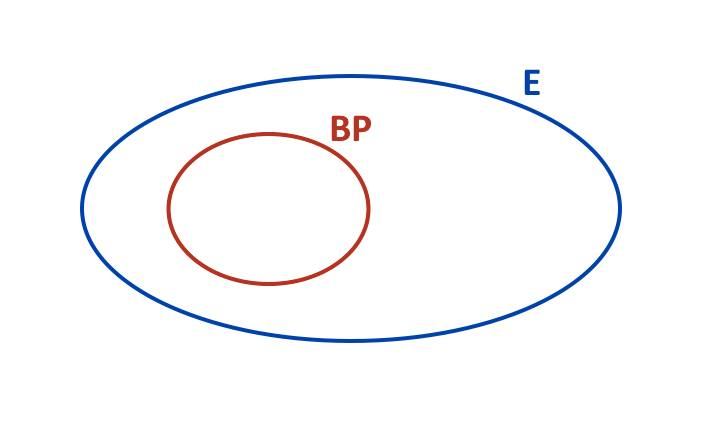
\includegraphics[scale=0.5]{Ensembles}
\end{figure}


\item INV 2 : La variable "depart" contient l'indice auquel nous avons démarré le tour courant du cadran.

\item INV 3 : La variable "memoire" contient l'élément que nous devons déplacer.

\item INV 4 : La variable "index" contient l'indice auquel nous devons déplacer l'élément contenu dans "mémoire".
\end{enumerate}



\subsubsection*{Condition d'arrêt}

H : i = |E|

\subsubsection{Triplet de Hoare-Manna}
\vspace{0.2cm}

\textbf{\{Pre\} INIT \{INV\}}
\vspace{0.2cm}

\textbf{Pre} :
\begin{enumerate}
 \item rotation = le nombre de rotation que l'on souhaite faire. 
 \item cadran un tableau non vide représentant l'état du cadran.
\end{enumerate}

\vspace{0.2cm}

\textbf{INIT} :

\begin{enumerate}

\item rotation = rotation\%cadran.length => Par la théorie du modulo, ne modifie pas le problème.

\item depart = 0 => Respecte bien INV 2 à l'initialisation : nous démarrons le premier tour à l'indice 0.

\item memoire = cadran[depart] => Respecte bien INV 3 : le premier élément à déplacer est celui à l'indice 0.

\item  index = rotation => Respecte bien INV 4 : nous voulons placer le contenu de "memoire" (càd l'élément à l'indice 0) à l'indice "rotation" du tableau.
        
\item int i = 0 => Respecte bien INV 1 : il y a 0 élément correctement placé.
\end{enumerate}
\vspace{0.3cm}

Nous retrouvons donc bien l'invarient à la fin de l'initialisation (en partant des préconditions). \\

\textbf{\{INV \&\& !H\} ITER \{INV\}}

Deux cas possibles :\\
\begin{enumerate}
\item Soit index == depart (cela signifie que nous avons réalisé un tour mais que, par !H, le travail n'est pas fini ; cela arrivera pgcd(rotation, |cadran|) fois, cfr. théorie du problème)
\begin{enumerate}

\item cadran[index] = memoire : cette opération réalise le dernier changement de ce tour. Cela permet de respecter INV 1 en plaçant correctement un élément de plus.
\item depart = depart + 1 : sachant, que (par INV 2), depart contenait l'indice de depart du tour qui est en cours, nous décalons l'indice de départ de 1, ce qui nous permet de commencer un nouveau tour à cet indice. Cela respecte donc INV 2. (Rem. : nous devons réaliser l'opération %|cadran| sur ce nombre pour ne pas sortir du tableau)
\item memoire = cadran[depart] : memoire retient le nouvel élément que nous devons déplacer, à savoir l'élément à l'indice de départ du nouveau tour. INV 3 est donc également respecté.
\item index = depart + rotation : nous respectons bien INV 4 en ce sens que l'indice auquel nous devons placer memoire est bien l'indice de départ du tour augmenté du nombre de rotations à effectuer. (Rem. : nous devons réaliser l'opération %|cadran| sur ce nombre pour ne pas sortir du tableau)
\item i++ : grâce au premier point de cette liste qui a placé correctement un élément supplémentaire, cette incrémentation respecte INV 1.
\end{enumerate}
\item Soit index != depart (cas "normal")\\
\begin{enumerate}
\item Nous plaçons le contenu de memoire (élément à déplacer) dans cadran[index] (indice où l'on doit placer l'élément) et l'ancien contenu de cadran[index] (nouvel élément à déplacer) dans memoire. Cela a pour effet de respecter INV 1 en plaçant correctement un élément supplémentaire et de respecter INV 3 en plaçant dans memoire l'élément suivant à déplacer.
\item index = index + rotation : cela respecte bien INV 4. (Rem. : nous devons réaliser l'opération %|cadran| sur ce nombre pour ne pas sortir du tableau)
\item INV 2 est respecté car nous ne modifions pas départ.
\item i++ ne contredit pas INV 1, de par le fait du premier point de cette liste qui a placé correctement un élément supplémentaire.\\
\end{enumerate}
\end{enumerate}

\textbf{\{INV \&\& H\} CLOT \{Post\}}


CLOT est vide, car nous avons modifié le tableau tout au long des itérations.
La seule partie de l'invariant utile ici est INV 1 qui nous dit que 0 $\le$ i $\le$ |BP| $\le$ |E|. De plus, H nous dit que i = |E|. Nécessairement, donc, |BP| = |E|, ce qui signifie qu'il y a autant d'éléments dans BP que dans E. Autrement dit, tous les éléments de E sont bien placés.
Nous respectons donc bien \textbf{Post}.

\section{Preuve du variant}


\end{document}